
\section{Adaptive Variable-Order SHE}



\begin{frame}{Adaptive Variable-Order SHE}

  \vspace*{-0.05cm}
  \begin{block}{Spherical Harmonics Expansion}
     \vspace*{-0.6cm}
      { \begin{align*}
	f(\mathbf x, \mathbf k, t) \simeq \sum_{l = 0}^L \sum_{m=-l}^l f_{l,m}(\mathbf x, E, t) Y_{l,m}(\theta, \varphi)
      \end{align*}}
     \vspace*{-0.6cm}
  \end{block}

  \begin{itemize}
   \item $(L+1)^2$ unknown functions $f_{l,m}(\mathbf x, E, t)$
   \item $L=0$ sufficient in equilibrium
   \item Higher-order expansions in active regions
   \item Therefore: Variable-order SHE:
      { \Large \begin{align*}
	f(\mathbf x_i, \mathbf k_n, t) \simeq \sum_{l = 0}^{L(\mathbf x_i, E_n)} \sum_{m=-l}^l f_{l,m}(\mathbf x_i, E_n, t) Y_{l,m}(\theta, \varphi)
      \end{align*}}
   \item How to choose $L(\mathbf x_i, E_n)$ in the simulation domain?
  \end{itemize}
     \vspace*{0.92cm}
\end{frame}





\begin{frame}{Adaptive Variable-Order SHE}
  
 \begin{block}{Motivation from Fourier series}

  \vspace*{0.6cm}
  \begin{minipage}{0.97\textwidth}
    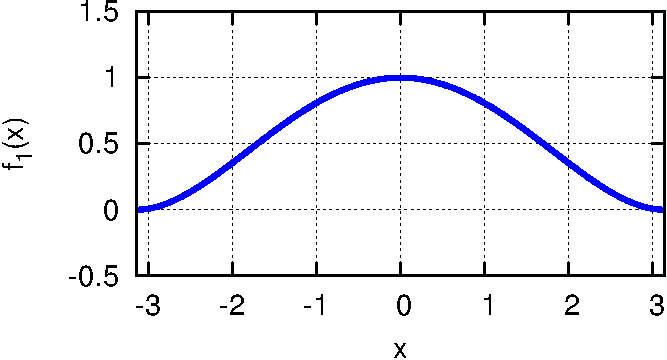
\includegraphics[width=0.45\textwidth]{fourier_f1} \hspace*{0.25cm}
    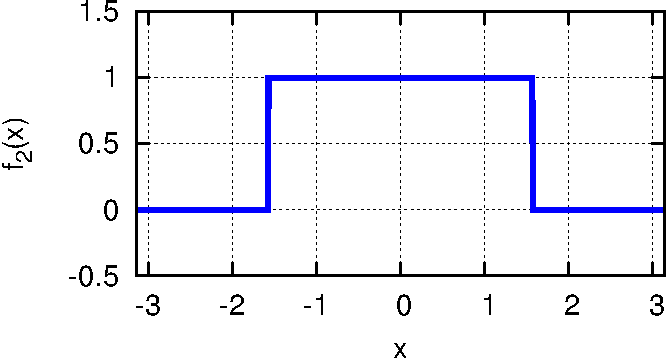
\includegraphics[width=0.45\textwidth]{fourier_f2} \hspace*{0.25cm} \newline

    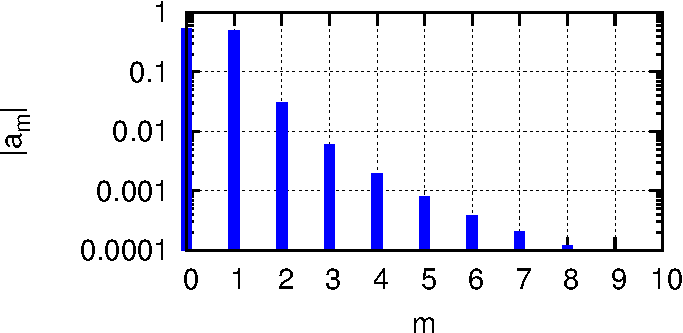
\includegraphics[width=0.45\textwidth]{fourier_coeff_1}\hspace*{0.25cm}
    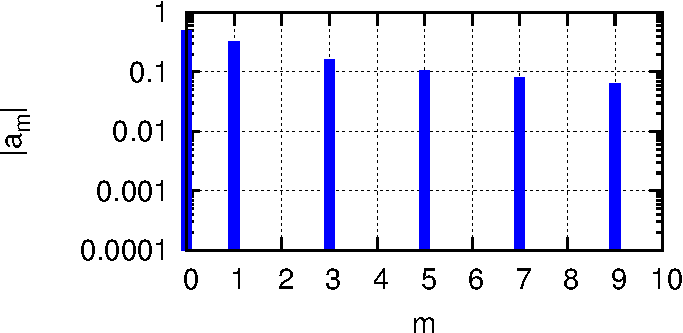
\includegraphics[width=0.45\textwidth]{fourier_coeff_2}
  \end{minipage}
 \end{block}

\end{frame}




\begin{frame}{Adaptive Variable-Order SHE}

 \fcolorbox{white}{white}{
  \begin{minipage}{0.1\textwidth}
    $L=1$ \\ 
    \vspace*{3cm} \\
    $L=3$
  \end{minipage}


  \begin{minipage}{0.4\textwidth}
  \begin{center} Error indicator:\\
    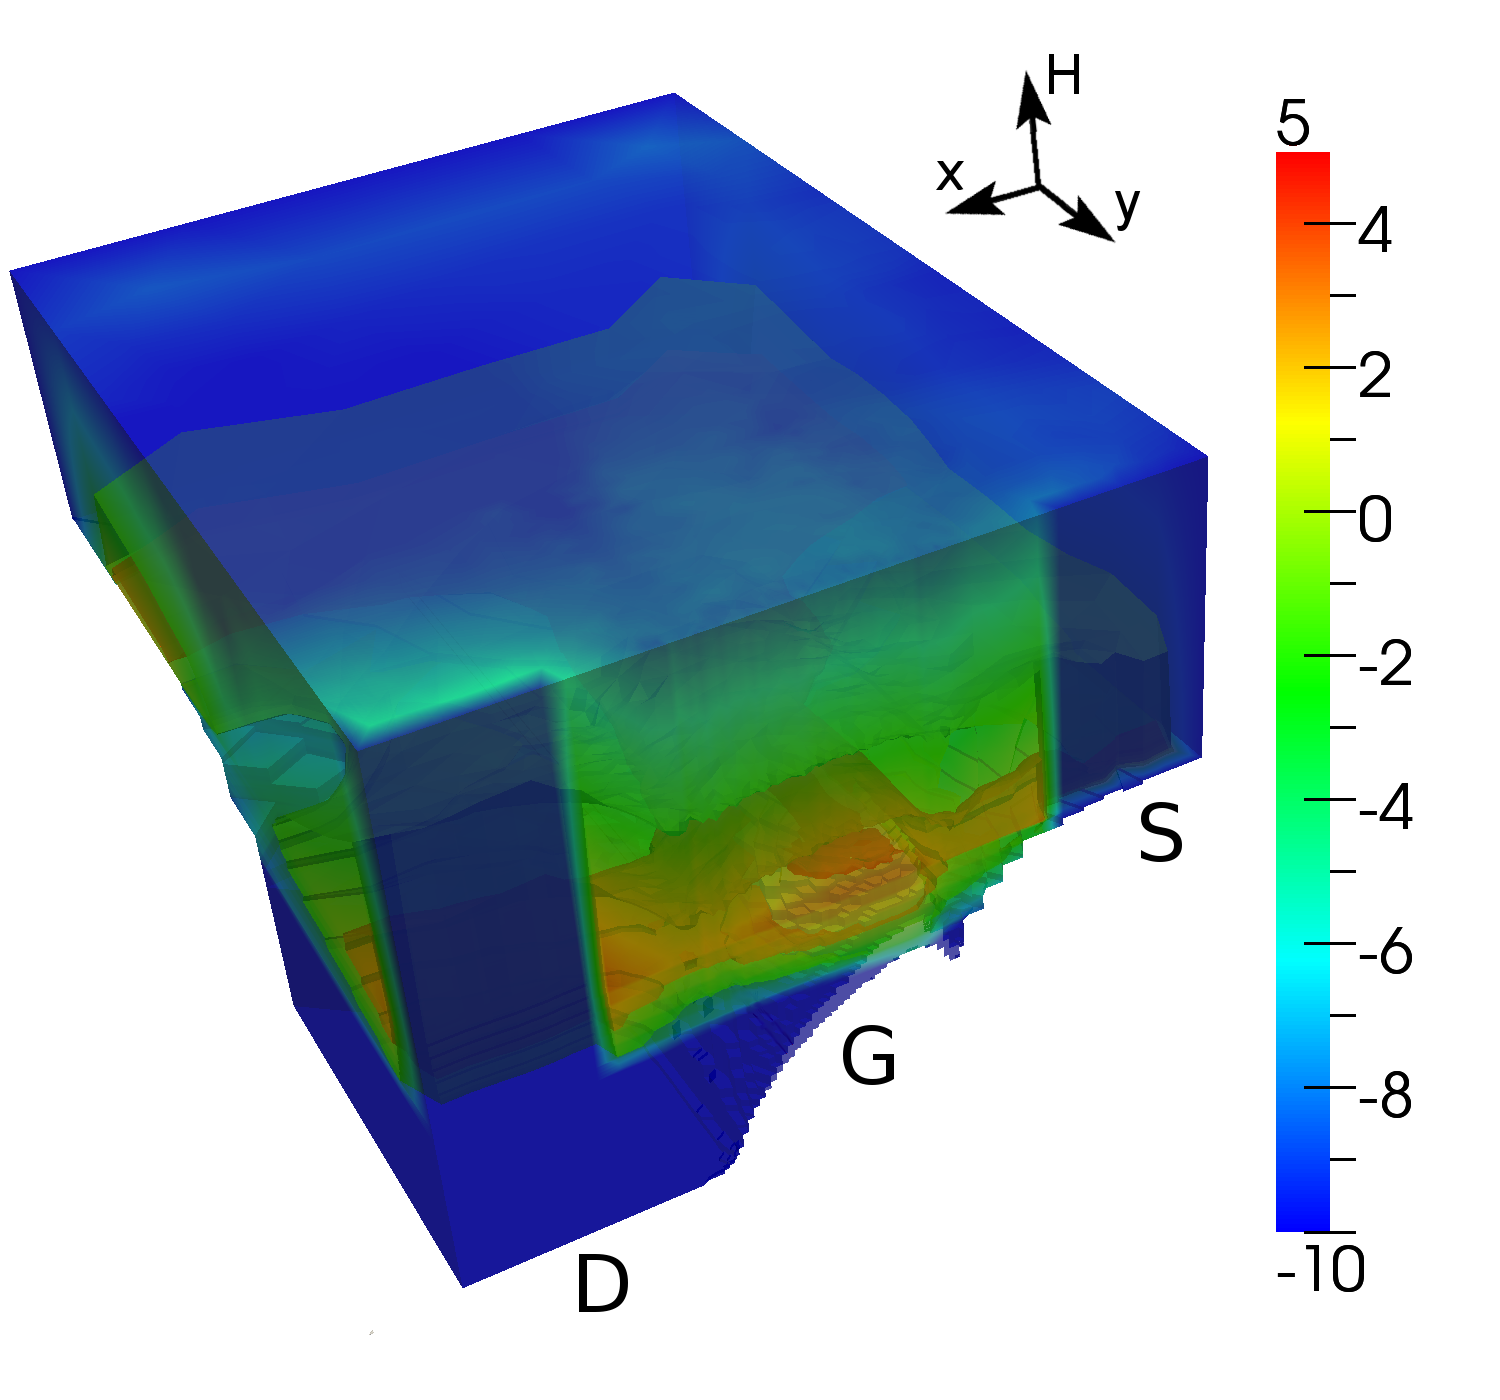
\includegraphics[width=0.9\textwidth]{mosfet-indicator-1} \\
    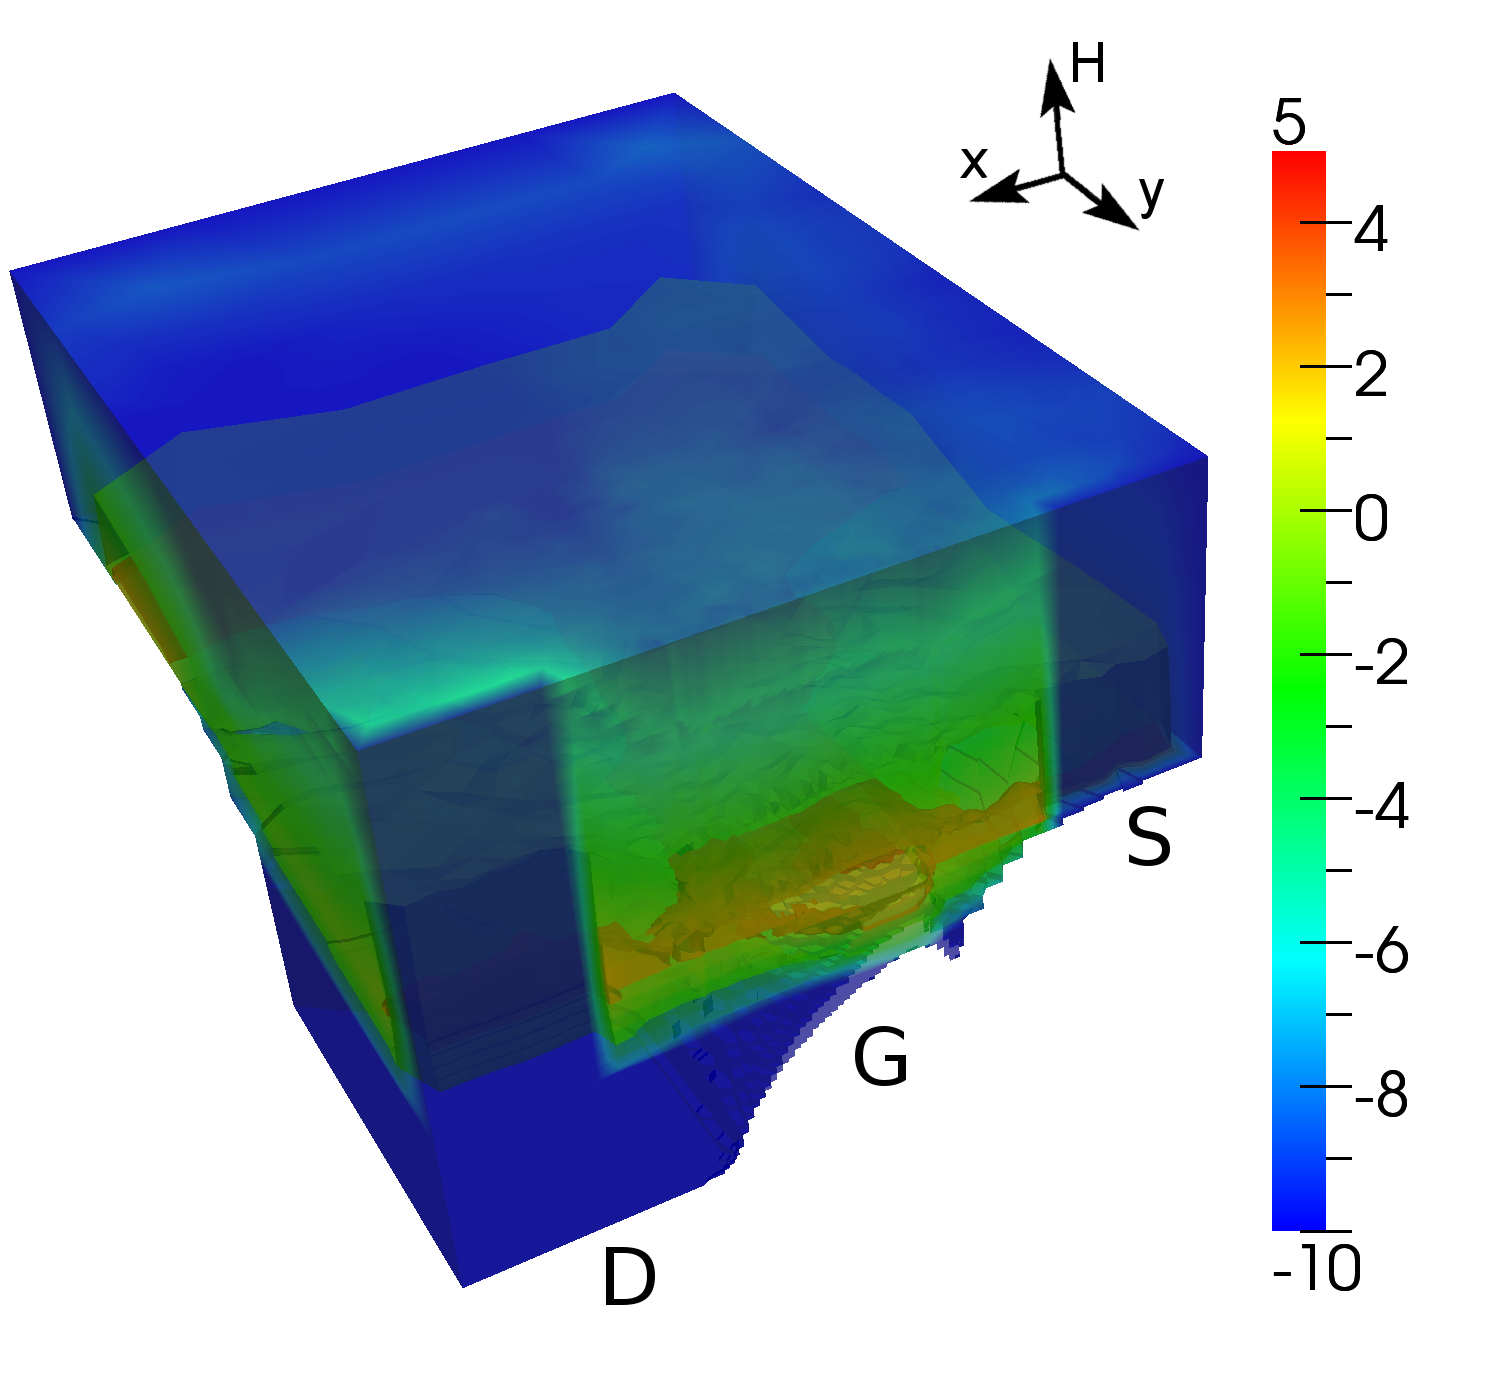
\includegraphics[width=0.9\textwidth]{mosfet-indicator-3}
  \end{center}
  \end{minipage}
  \hspace{0.5cm}
  \begin{minipage}{0.4\textwidth}
  \begin{center} Expansion order:\\
    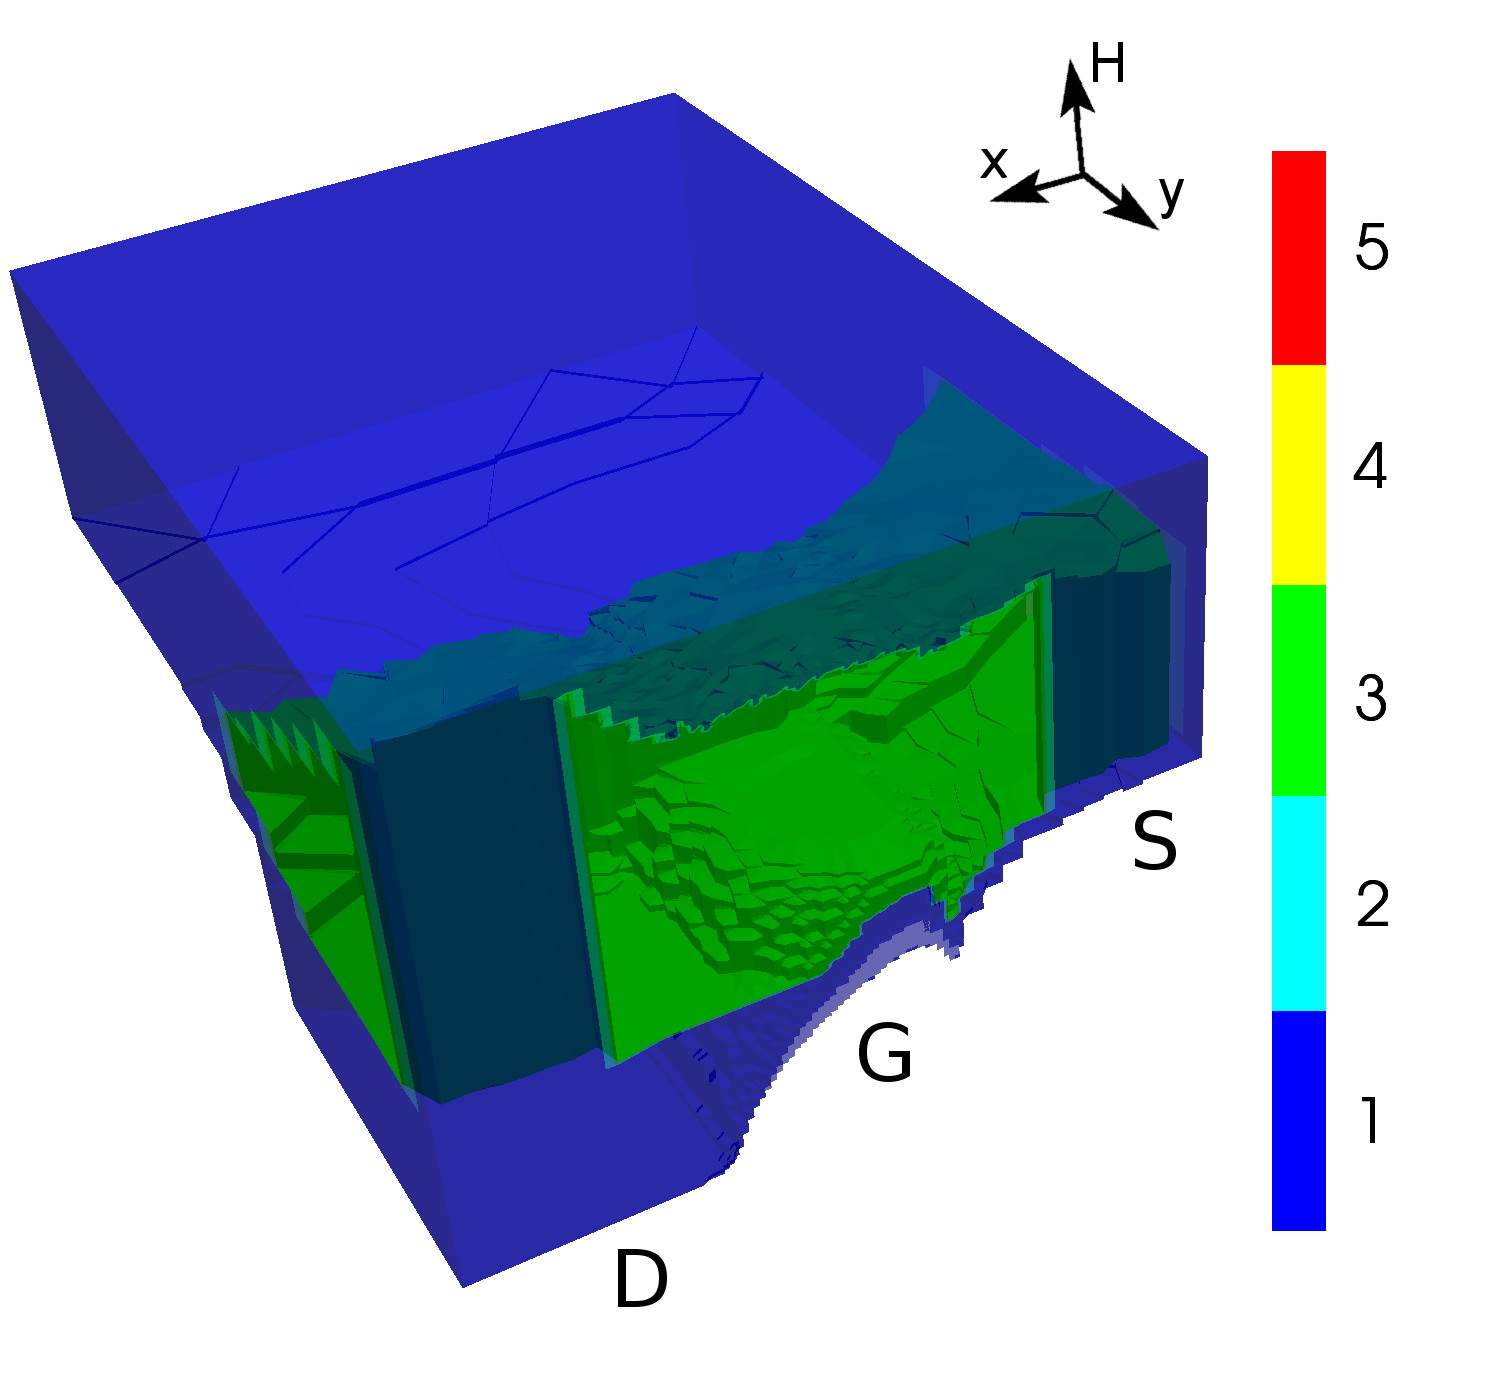
\includegraphics[width=0.9\textwidth]{mosfet-order-1} \\
    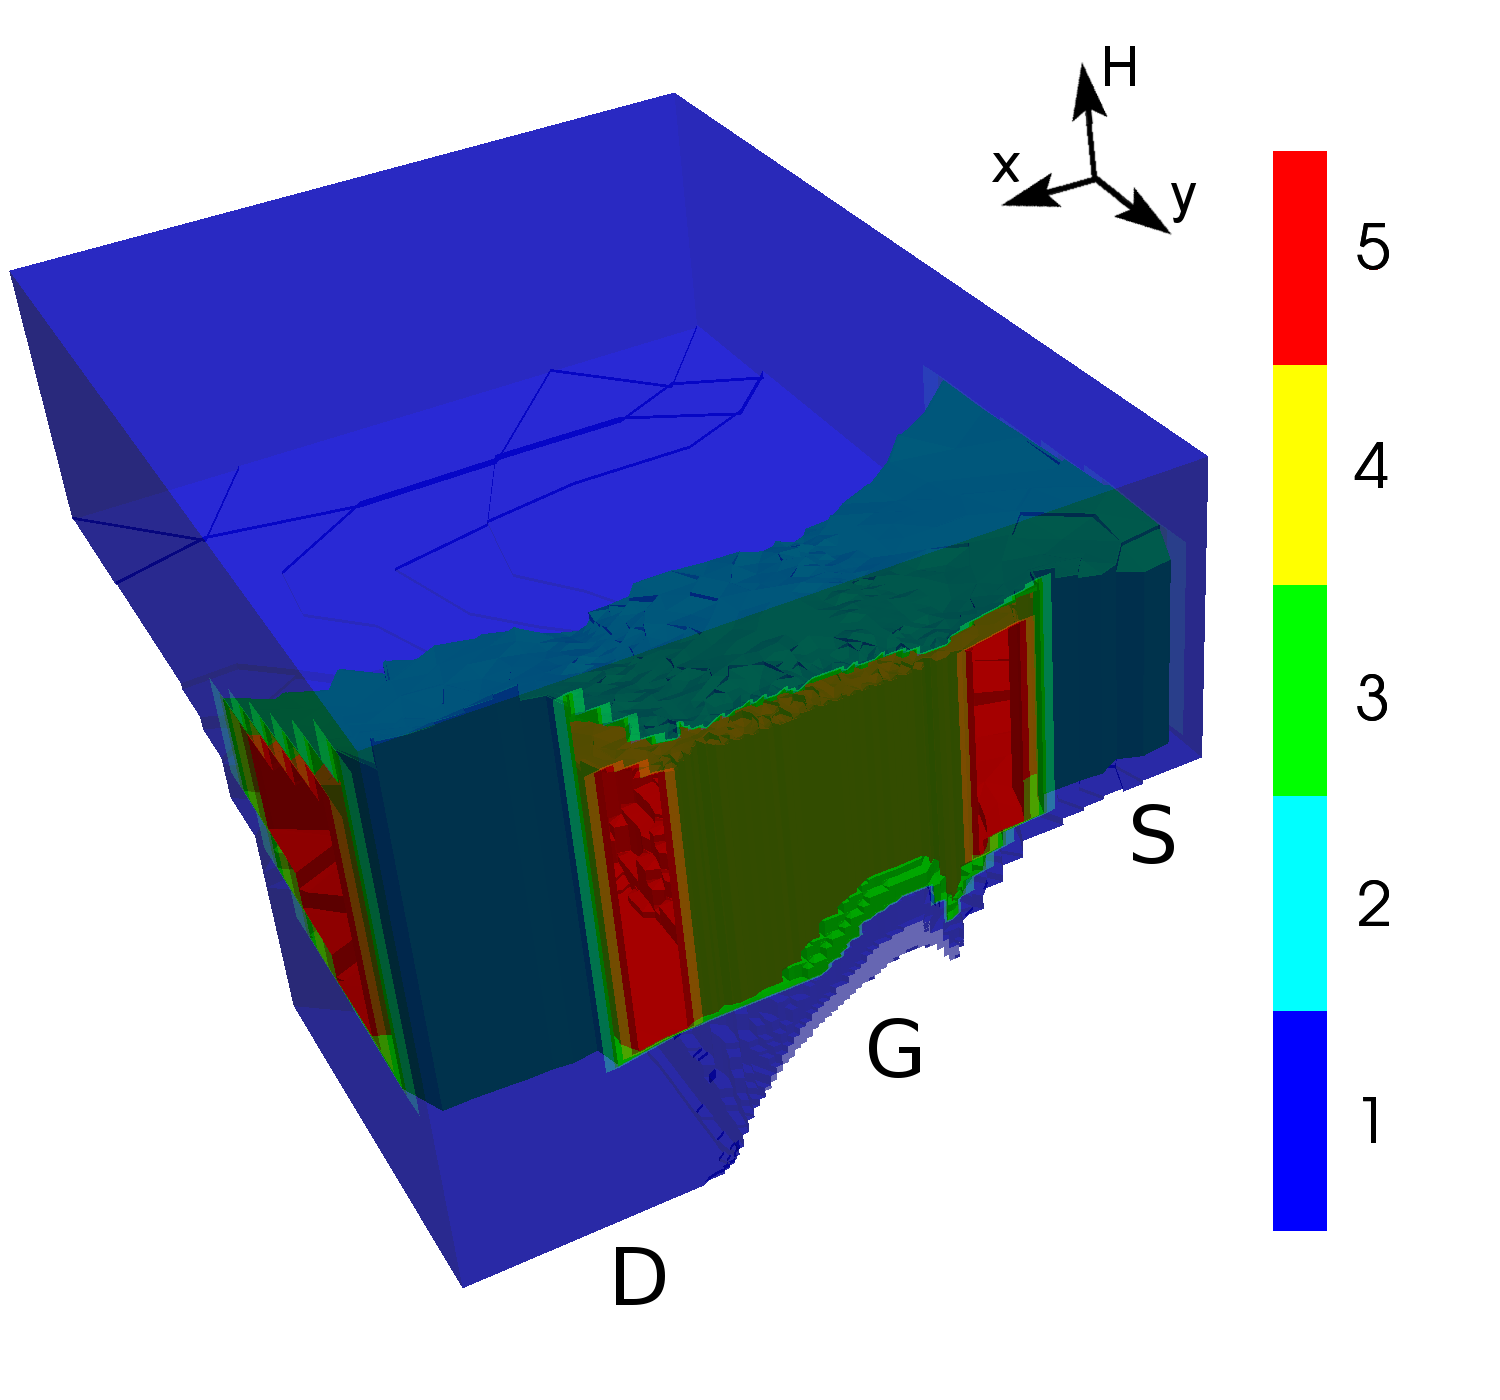
\includegraphics[width=0.9\textwidth]{mosfet-order-3}
    %\vspace*{1cm}
  \end{center}  
  \end{minipage}
  \hspace{2.5cm}
 } %end of fcolorbox

%   \vspace*{-0.5cm}
\end{frame}


\begin{frame}{Adaptive Variable-Order SHE}
  \vspace{-0.3cm}
  \begin{center}
   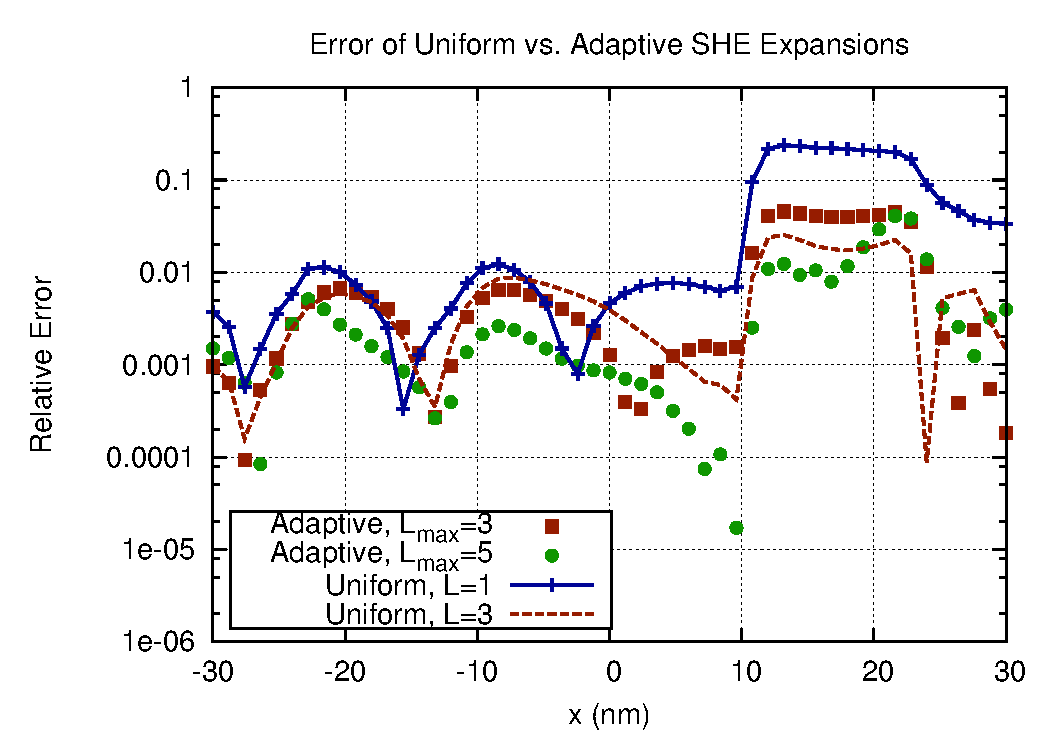
\includegraphics[width=0.75\textwidth]{mosfet-energy-error}
  \end{center}
  \vspace{-0.4cm}
  \begin{center}
   %\begin{itemize}
    %\item 
      $L=3$: $\mathbf{306\, 261}$ instead of $\mathbf{\hphantom{1}\, 476\, 061}$ unknowns (factor $\mathbf{1.5}$) \\
    %\item 
      $L=5$: $\mathbf{606\, 671}$ instead of $\mathbf{1\, 146\, 120}$ unknowns (factor $\mathbf{1.9}$)
   %\end{itemize}
  \end{center}
%   \vspace*{-0.5cm}
   
\end{frame}

% \begin{frame}{Summary}
%  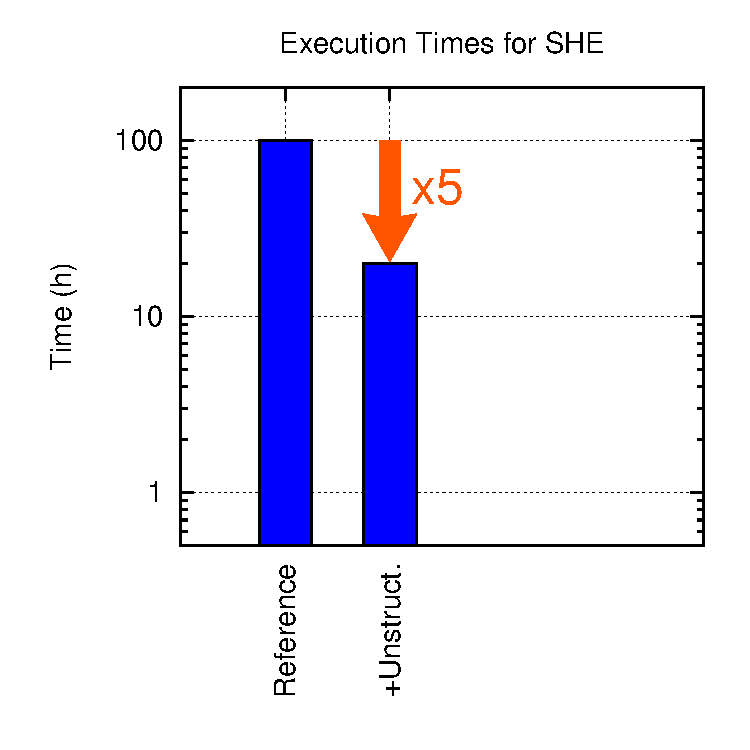
\includegraphics[width=0.49\textwidth]{summary-exec-2}
%  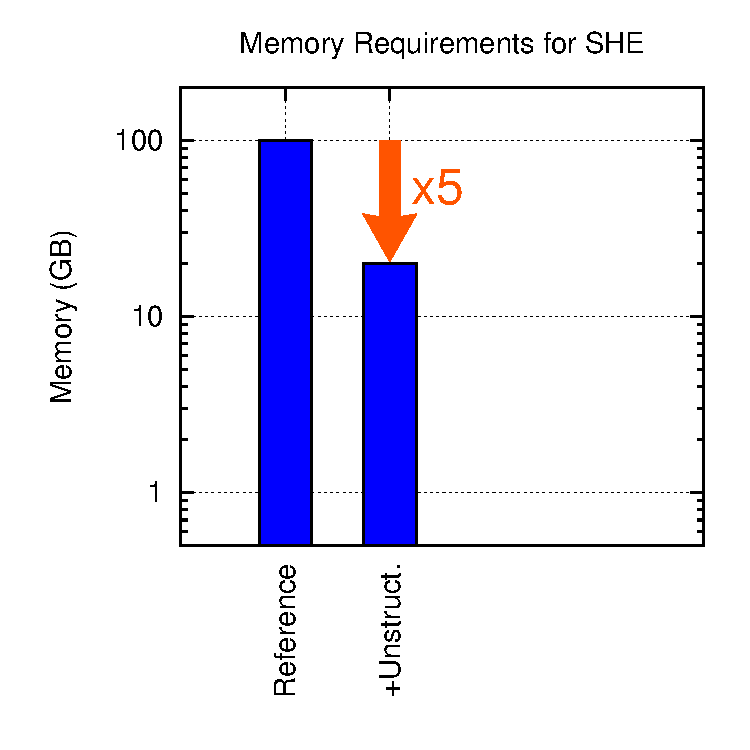
\includegraphics[width=0.49\textwidth]{summary-memory-2}
% \end{frame}

\begin{frame}{Summary}
  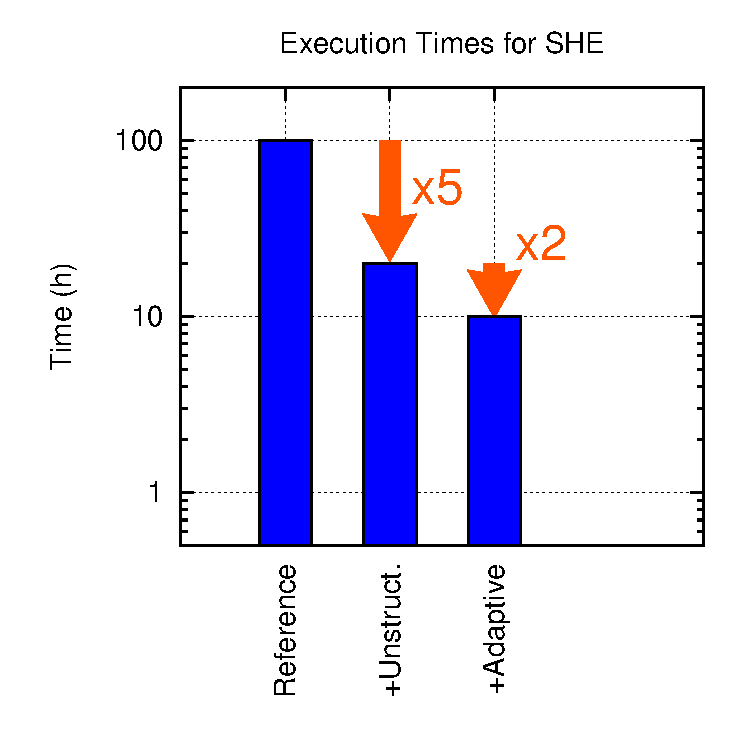
\includegraphics[width=0.49\textwidth]{summary-exec-3}
  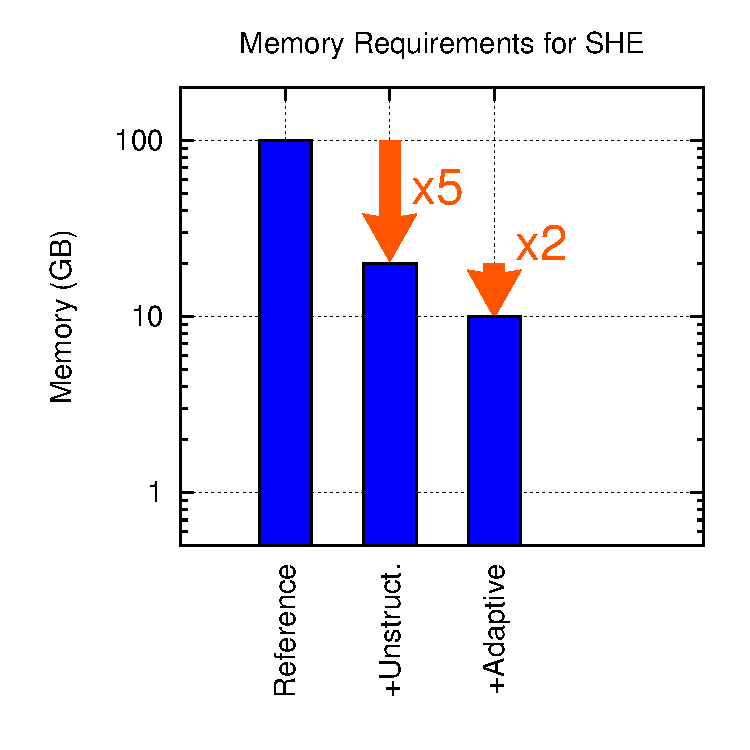
\includegraphics[width=0.49\textwidth]{summary-memory-3}
\end{frame}

